\chapter[The breakdown process]{The breakdown process}

In this chapter the detected effects of the breakdowns and an overview of the theoretical models will be presented. The setups for studies on the vacuum breakdown physics will not be presented indeed, and a good review can be found in \cite{Kovermann:1330346}. The reason is that using the setup object of this work it is just possible to have a glimpse on the beam effect, but not perform the measurements that are normally carried out in breakdown physics. This is caused by the beam presence, that make the majority of the sensors that are normally used blind or not installable.

The large amount of parameters that play a role in the breakdown process makes researching in this field very complicated. For the same reason is also very difficult the comparison of different experiments. This situation has led to a division in the scientific community about the theoretical description of the phenomenon.

Researchers anyway converge on the fact that, at low pressures, the vacuum arc initiation process is dependent by the surface and material properties, but is independent form the pressure itself \cite{alpert:triggers}.

Strong efforts in pursuing the understanding of the phenomenon have been made so far, with the result of the improvement of the maximum gradient achievable in accelerating structures and the development of the first simulation codes \cite{Insepov:1373092}.



\section[Detected effects of breakdowns in accelerating cavities]{Detected effects of breakdowns in accelerating cavities}

Most of the theories about breakdown converge on the fact that the breakdown and the field emission are different phenomena. While the field emission is always present, the breakdown of the field is a rare event, and depends by different causes, first of all the material.

Therefore in the detection of the breakdown a background current emitted by FE is always present, but on top of that are appreciable during the breakdown \cite{Wuensch:583549}:

\begin{itemize}
\item RF pulse reflection: after the breakdown the incoming power is reflected back
\item X-ray production: an isotropical emission of X-rays is appreciable. Unfortunately passing through the structure any information carried by the spectrum is lost
\item Visible light emitted by the arc
\item Current bursts exiting the cavity
\item Vacuum level spikes: this effect fades while the conditioning continues. Will be discussed in the section 3.3 
\end{itemize}
Other effects, such as shock waves, have also been appreciated \cite{Rajamaki:2143815}. 

In figure \ref{RFandBPM} is reported an RF pulse and the current burst measured with the setup used in this work during a run without beam. It is clearly visible the fall of the transmitted power and the raise of the reflected one. Also comparing the area of the two signals to the previous pulse, it's clear that a significant amount of energy is missing. This is imputable to the energy necessary to sustain the plasma that forms during the breakdown. On the left it is visible qualitatively the current burst emitted by the cavity on the downstream BPM. It has to be kept in mind that the BPM is placed far from the exit of the cavity, resulting in a poor charge detection because of the small solid angle covered; also the proper device to collect the emitted charge is a Faraday Cup, which cannot be installed in this setup because the beam pipe needs to be free. 


\begin{figure}[h]
\centering
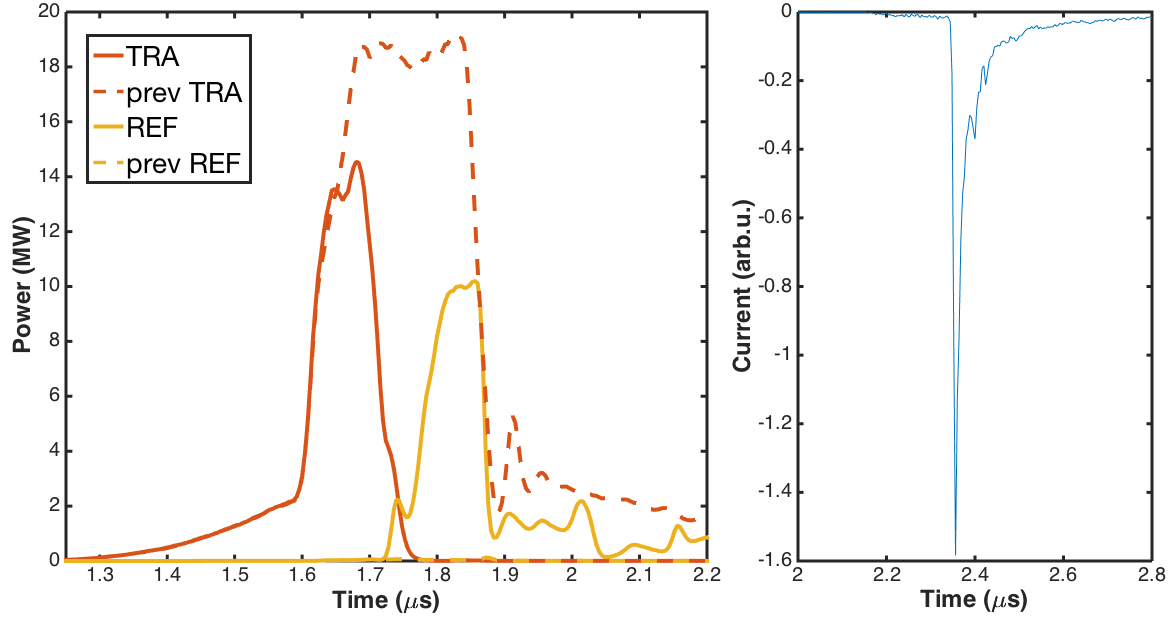
\includegraphics[scale=0.33]{pictures/RFandBPM.png}
\caption{RF signals of a breakdown event (left) and burst of current emitted, detected by a BPM (right). In the left plot it is clearly visible the fall of the transmitted power (solid red) and the raise of the reflected power (solid yellow). The RF signals of the previous pulse, so without breakdown, are reported dashed. Note that the time scale in the two plots are not comparable.}
\label{RFandBPM}
\end{figure}




\section[Vacuum arc process description]{Vacuum arc process description}

A fully satisfactory theory to describe the breakdowns has not been formulated yet, but the scientific community produced a number of models to describe the breakdown mechanism and initiation, summarised in \cite{soviet:1983,davies:triggers}. Most of them converge on the role that the field emission would have in triggering the breakdown, even if irrefutable  evidences have to be shown yet.

\subsubsection[Triggers]{Triggers}

The surface of the cathode is not completely flat, but presents some asperities that enhance the field emission as pointed out in chapter 2. This process leads to the formation of hot zones called \textit{field emitters} where the local electric field is enhanced of a factor $\beta$ because of the geometry and the current emitted is therefore increased (see figure \ref{BD_rocess}, box a). 

The current flow through the tip heats it up, modifying its physical properties and applying a tensile stress. Theories diverge on the process that takes place at this point: some prepend for the heating up of the tip up to the fusion, like \cite{Grudiev:newLoc}; others on the cracking process of the tip due to the tensile stress applied by the enhanced electric field, which gets comparable to the tensile strength of the material around fields of $10$ GV/m  \cite{Insepov:1373092}.

It is in any case possible that during this process the shape of the tip gets modified, enhancing the $\beta$ factor even more.


\subsubsection[Plasma initiation]{Plasma initiation}

The peculiarity of the breakdown is that is a phenomenon that takes place in vacuum, and has been detected even at large gaps. According to many experimental results, the plasma is created from the cathode material (regardless on how it got emitted from the surface). The cathode material form a neutral gas surrounding the tip, that gets ionised by the electrons emitted by field emission (see figure \ref{BD_rocess}, box b). In this first phase the ions created in this manner drift under the effect of the space-charge effect. The plasma initiation last only few ns.

Spectroscopical measurements of the light emitted by the plasma have shown that the plasma is formed of ions with various charge and electrons. The DC spark system at CERN showed that the plasma formed by copper cathodes present ionisation levels up to Cu$^{3+}$. \cite{find quote}


\subsubsection[Plasma evolution]{Plasma evolution}

The ion density of the plasma over the emitter result in the establishment of a sheath potential, which enhances the electrical field even more, provoking an exponential  increase of the field-emitted current. The current emitted reaches values of several A/$\mu$m$^2$, determining the melting of the emitter (see figure \ref{BD_rocess}, box c).

The molten metal becomes part of the plasma, that expands modifying temperature and density. The sheath potential gets modified as well. After an expansion process, where part of the plasma interact with the surface, determining erosion, the greatest part of the ions recombinate with the electrons determining an intense optical emission.


\subsubsection[Cratering phase]{Cratering phase}

During the last plasma expansion, the ions impacting on the surface are expected to create new field emitters. The emitters will melt and result in an explosive emission because of the high field provoked by the sheath potential (see figure \ref{BD_rocess}, box d). 

The full arc is expected to continue up to the end of the RF pulse. Next the plasma is expected to disappear for expansion cooling or recombination. All the process result in a surface damage in the emitter zone and the surroundings. If in the damaged zone other asperities have been created, them will trigger new breakdowns according to the new value of $\beta$ (see figure \ref{BD_rocess}, box e, f). 

In figure \ref{SEM_crater} a photograph of a crater is shown, taken using a scanning emission microscope.
\begin{figure}[h]
\centering
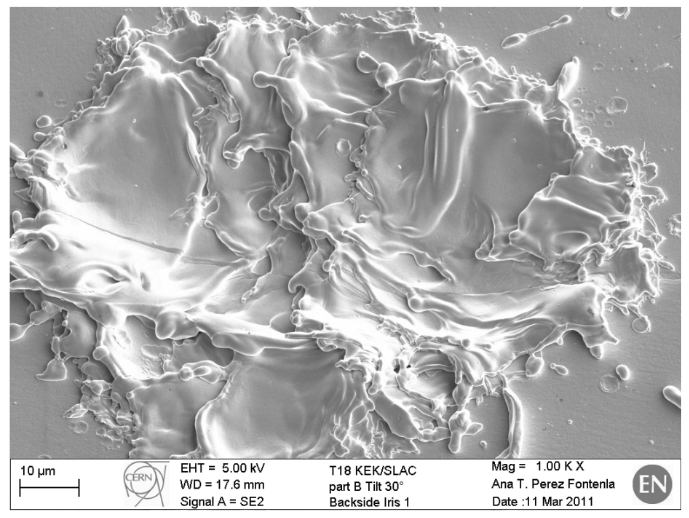
\includegraphics[scale=0.5]{pictures/crater}
\caption{Crater provoked by a breakdown in an X-band RF accelerating cavity \cite{Wuensch:advaces}}
\label{SEM_crater}
\end{figure}



\begin{figure}[h]
\centering
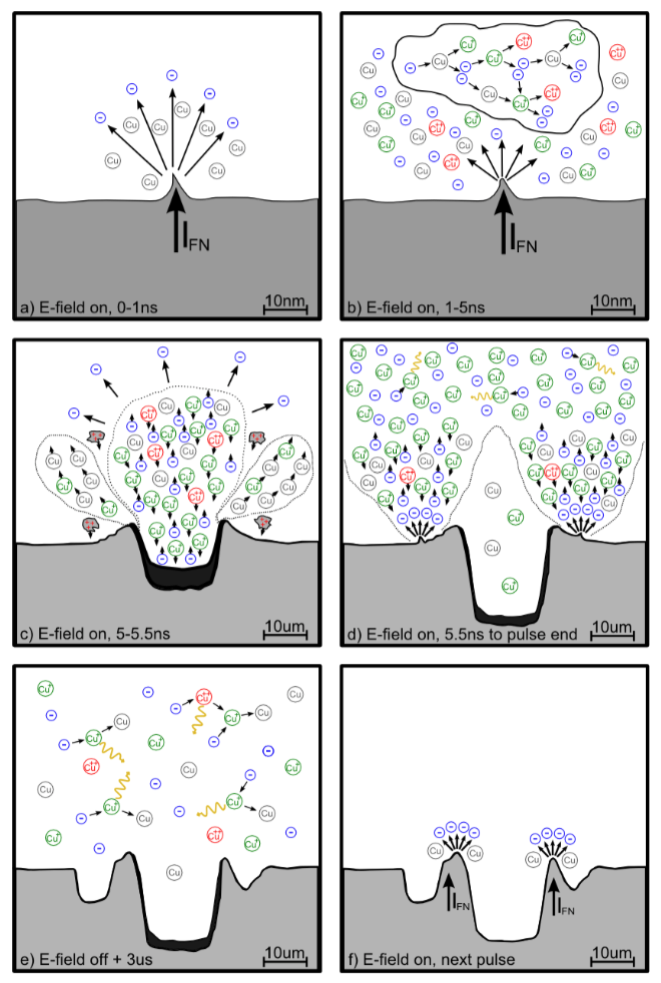
\includegraphics[scale=0.4]{pictures/BD_process}
\caption{Breakdown stages in chronological order. From \cite{Kovermann:1330346}}
\label{BD_rocess}
\end{figure}


\section[Breakdown rate scaling law]{Breakdown rate scaling law}

The interest on breakdowns in accelerator physics arose in order to avoid as much as possible perturbations of the beam. A key parameter of an accelerating cavity is the breakdown rate (BDR).

The breakdown rate is the number of breakdowns that happens per number of RF pulses. Measuring the BDR of a cavity means to measure a probability, that makes sense only if the cavity has been tested with a sufficient number of pulses. 

According to the latest developments, the BDR follows the scaling law
\begin{equation}
BDR \propto E^{30}_a \tau^5_p 
\end{equation}
where E$^{30}_a$ is the accelerating gradient, and $\tau$ the pulse length  \cite{Wuensch:advaces}.

This scaling law allows to compare the performance of different accelerating structures and different tests. It is important to underline that the scaling law was deduced by the results of the experiments executed so far, but does not imply any kind of assumption on the physics of the breakdown process.




\section[Influence of the conditioning process]{Influence of the conditioning process}

It has been mentioned how the trigger mechanism of the breakdowns seems to depend from the condition of the surface of the accelerating cavity. In order to reach the low breakdown rate that is affecting the performance of the linear colliders, two strategies have been used:
\begin{enumerate}
\item Refining of the production and assembly techniques of the cavites
\item Conditioning the structure with a series of RF pulses increasing the power gradually and keeping the breakdown rate limitated
\end{enumerate}
The current production procedure for the structures for CLIC is outlined in~\cite{CLIC:cdr}. The conditioning process is a more complicated matter. 

The conditioning of an accelerating structure is conducted applying repeatedly RF power pulses at a fixed pulse length, while keeping the breakdown rate limited under a certain threshold. This is realised modifying the input power, that gets raised if for a period no breakdown happens, or lowered if the breakdown rate gets to high. When the power goal has been reached, the pulse length is increased, and the process restarts with low power pulses.

The process terminates when both the power and the pulse length goal has been reached. In many experiments the breakdown rate has exhibited an exponential decrease with the conditioning time. The conditioning of a structure may last up to 3-4 months to reach the design breakdown rate. Understanding the process and find the right conditioning strategy gets then fundamental, and many efforts have been made in this sense. The surprising result is that the conditioning process proceeds with the number of RF pulses rather than the number of breakdowns happened \cite{Degiovanni:2065711}.

The physical process that provokes breakdown might change as long as the conditioning goes on. According to recent results \cite{Wuensch:583549}, the vacuum level increase, that takes place during a breakdown, fades as time goes by. This effect is probably addressable to the stimulated desorbtion \cite{soviet:1983}, that provokes a gradual release of the absorbed gas into the metal, that gets pumped out. This effect is triggered in presence of strong electric fields only, the same fields that are involved during the breakdown process. The contribution of the desorbed gas is still not clear anyway. Another possible effect is the presence of dust particles on the surface, that gets cleaned up as conditioning continues.

A review of the conditioning algorithm used, and the conditioning history of the accelerating cavity used in this work can be found in \cite{Degiovanni:1742280}










